\documentclass[tikz,border=1pt]{standalone}
\usepackage[T1]{fontenc}
\usepackage[utf8]{inputenc}
\usepackage{amsmath,amssymb,pifont}

% https://tex.stackexchange.com/q/130232/13304 for 
% circled numbers

% ACM
\usepackage[tt=false, type1=true]{libertine}
\usepackage[varqu]{zi4}
\usepackage[libertine]{newtxmath}

% IEEE
%\renewcommand{\sfdefault}{phv}
%\renewcommand{\rmdefault}{ppl}
%\renewcommand{\ttdefault}{pcr}
%\usepackage{mathptmx}

\usetikzlibrary{bending,
	calc,
	fit,
	shapes.arrows,
	shapes.geometric,
	decorations.pathreplacing,
	shadows,
	arrows.meta,
	backgrounds,
	positioning,
	hobby
}

\usepackage{pgfplots}
\usepgfplotslibrary{colormaps}
\tikzset{
	fill-color/.style={
		color of colormap={#1},
		draw=.!80!black,
		fill=.!60!white,
		text=black,
	},
	draw-color/.style={
		color of colormap={#1},
		draw=.,
		text=black
	},
	mydashed/.style={dash pattern=on 6pt off 4pt},
	module/.style={rounded corners, minimum width=1cm, minimum height=.75cm,ultra thick,anchor=north,text=black,align=center,},
	state/.style={color of colormap={#1},ellipse, top color=white, bottom color=.!35,draw, text=black, inner xsep=0pt},
}
\begin{document}
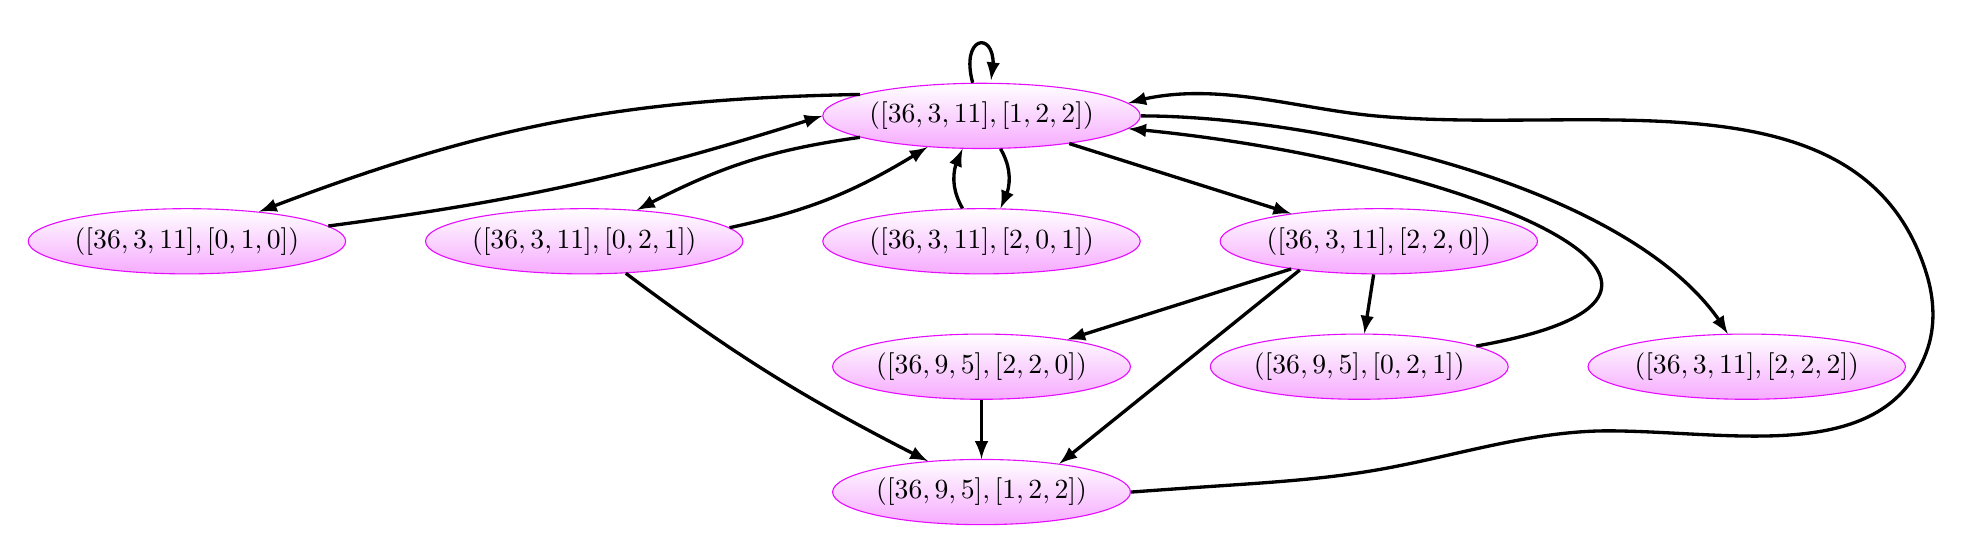
\begin{tikzpicture}[node distance=0.75cm and 1 cm,-latex, /pgfplots/colormap/cool,]


% graph

\node[state=950] (n1) at (0,0) {$([36, 3, 11], [1, 2, 2])$};
\node[state=950, below=of n1] (n2) {$([36, 3, 11], [2, 0, 1])$};
\node[state=950, right=of n2] (n3) {$([36, 3, 11], [2, 2, 0])$};
\node[state=950, left=of n2] (n4) {$([36, 3, 11], [0, 2, 1])$};
\node[state=950, left=of n4] (n5) {$([36, 3, 11], [0, 1, 0])$};

\node[state=950, below=of n2] (n6) {$([36, 9, 5], [2, 2, 0])$};
\node[state=950, right=of n6] (n7) {$([36, 9, 5], [0, 2, 1])$};
\node[state=950, right=of n7] (n8) {$([36, 3, 11], [2, 2, 2])$};

\node[state=950, below=of n6] (n9) {$([36, 9, 5], [1, 2, 2])$};

% connections

\path (n1) edge [loop above, very thick,->, >=latex] (n1);

\path (n1) edge [bend left, very thick] (n2);
\path (n2) edge [bend left, very thick] (n1);

\path (n1.190) edge [bend right=10, very thick] (n4);
\path (n4) edge [bend right=10, very thick] (n1.210);

\path (n1.170) edge [bend right=10, very thick] (n5);
\path (n5) edge [bend right=5, very thick] (n1.180);

\path (n3) edge [ very thick] (n6);
\path (n3) edge [ very thick] (n7);
\path (n1) edge [out=0, in =120, very thick, looseness=0.7] (n8);

\path (n7) edge [out=10, in =-5, very thick, looseness=2] (n1);

\path (n1) edge [ very thick] (n3);
\path (n6) edge [ very thick] (n9);
\path (n4) edge [bend right=5, very thick] (n9.150);

\draw[very thick] 
(n3.200)
--
(n9.20);

\draw[very thick] 
(n9.0)
to[curve through={(3,-4.7) .. 
	(5,-4.5) .. 
	(8,-4) ..
	(12,-3) ..
	(12,-2).. 
	(5,0) ..
	(2,0.2)
}
]  
(n1.5);

\end{tikzpicture}
\end{document}